\documentclass[a4paper,10pt]{scrreprt}
%\documentclass[a4paper,10pt]{scrartcl}

\usepackage[utf8]{inputenc}
\usepackage[german]{babel}
\usepackage[pdftex]{graphicx}
\usepackage{listings}
\usepackage{color}
\usepackage{amssymb}
\usepackage{marvosym}
\usepackage{amsmath}
\usepackage{array}
\usepackage{geometry}
\usepackage{listings}
\usepackage{upgreek}
\usepackage{color}
\usepackage{gensymb}

\geometry{verbose,tmargin=2cm,bmargin=2cm,lmargin=2cm,rmargin=2.5cm,headheight=80pt}
\newcolumntype{L}[1]{>{\raggedright\arraybackslash}p{#1}} % linksbündig mit Breitenangabe
\newcolumntype{C}[1]{>{\centering\arraybackslash}p{#1}} % zentriert mit Breitenangabe
\newcolumntype{R}[1]{>{\raggedleft\arraybackslash}p{#1}} % rechtsbündig mit Breitenangabe
\newcommand{\tabitem}{~~\llap{\textbullet}~~}

\newcommand{\pic}[1]{
  \begin{figure*}[ht!]
    \centering
    \includegraphics[scale=0.6]{pics/{#1}}
  \end{figure*}
}

\newcommand{\f}{\noindent\textbf}
\newcommand{\ku}{\textit}
\newcommand{\zb}{z.B.\ }
\newcommand{\ia}{i.A.\ }
\newcommand{\ua}{u.a.\ }
\newcommand{\idr}{i.d.R.\ }

\title{Eingebettete Systeme}
\author{A. Löffler, C. Hempfling}
\date{\today}

\pdfinfo{%
  /Title    ()
  /Author   ()
  /Creator  ()
  /Producer ()
  /Subject  ()
  /Keywords ()
}

\begin{document}
\maketitle

\begin{chapter}{Kapitel}
 \section*{Chapter 1.1}
 \f{Definition Eingebettetes System:}
 \vspace*{3pt}
 
 \noindent \ku{Ein eingebettetes System ist ein informationsverarbeitendes System bestehend aus Hardware und Software, das in einem technischen Gesamtsystem eingebettet 
 ist, dessen primärer Zweck nicht das Verarbeiten und Aufbereiten von Information ist.}\\
 \vspace*{5pt}
 
 \noindent Durch die zunehmende Komplexität hat sich der Entwurf eingebetteter Systeme von analogen Schaltungen und Assemblerprogrammen auf einfachen 
 Mikrokontrollern weg zum Problem hin entwickelt, komplexe Hardware/Software Systeme mittels leistungsfähiger Werkzeuge zu entwickeln und zu optimieren.
 \vspace*{5pt}
 
\begin{center}
 \begin{tabular}{|C{2cm}|C{4cm}|C{4.5cm}|}
  \hline 
  & \f{Eingebettetes System} & \f{konventioneller Rechner} \\ \hline 
  \f{Funktion} & \ku{feste Funktion}: zum Zeitpunkt des Entwurfs ist die Funktion, die das System übernehmen soll, bekannt & \ku{universell und offen}: zum 
  Zeitpunkt des Entwurfs sind die Funktionen, die das System übernehmen soll, weitgehend offen \\ \hline 
  \f{Verhalten} & \ku{reaktives Verhalten}: das System muss auf Aktionen der Umgebung unter festen zeitlichen Bedingungen reagieren & \ku{interaktives Verhalten}:
  das System sollte mit der Umgebung unter sehr losen zeitlichen Bedingungen interagieren \\ \hline 
  \f{Design} & \ku{Co-Design}: Hardware und Software werden aufeinander abgestimmt, entwickelt und optimiert & \ku{unabhängiges Design}: Hardware und Software 
  werden getrennt voneinander entwickelt und unabhängig voneinander optimiert \\ \hline 
 \end{tabular}
\end{center} 

\begin{itemize}
 \item aber auch konventionelle Computer haben eingebettete Systeme (z.B. Grafik-, Netzwerkkarte)
 \item die beiden wichtigsten Merkmale für eingebettete Systeme sind: 
 \begin{enumerate}
  \item reaktives Verhalten unter Echtzeitbedinungen
  \item gleichzeitige Entwicklung von Hardware und Software
 \end{enumerate}
 \item die Entscheidung, welche Funktionen in Hardware und welche in Software auf einem oder mehreren Mikrokontrollern realisiert werden, fällt oft sogar während 
 der Entwicklung und Optimierung des Entwurfs
\end{itemize}

\f{Abstraktionsebenen}:
\begin{figure}[!ht]
 \centering
 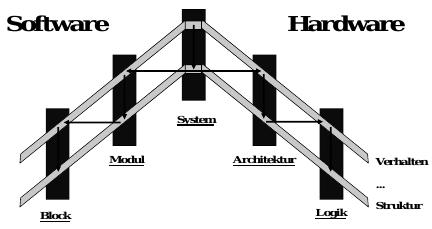
\includegraphics[scale=0.89]{pics/abstraktionsEbenen}
\end{figure}

\f{Abstraktionsebenen -- Software-Bereich}:
\begin{itemize}
 \item \ku{Modul}: die Modulebene gehört zum Softwarebereich. Die Modelle der Modulebene beschreiben komplexe Funktionen und ihre Interaktionen.
 \item \ku{Block}: die Blockebene gehört ebenfalls zum Softwarebereich. Die entsprechenden Modelle beschreiben Programme bis hin zu Instruktionen, die auf der 
 zugrundeliegenden Rechnerarchitektur elementare Operationen ausführen.
\end{itemize}

\f{Abstraktionsebenen -- Hardware-Bereich}:
\begin{itemize}
 \item \f{Architektur}: die Architekturebene gehört zum Hardwarebereich. Die Modelle dieser Ebene beschreiben kommunizierende Blöcke, die alle nebenläufig 
 komplexe Operationen ausführen.
 \item \f{Logik}: die Logikebene gehört ebenfalls zum Hardwarebereich. Die Modelle dieser Ebene beschreiben verbundene Gatter und Register, die Boolesche 
 Funktionen berechnen.
\end{itemize}

\f{Modell}:
\vspace*{3pt}

\noindent Unter einem Modell versteht man die formale Beschreibung eines Systems (oder Teilsystems). Wie genau ein Modell ein System beschreibt, hängt von der 
entsprechenden Abstraktionsebene ab. Man unterscheidet \idr zwischen 
\begin{itemize}
 \item \f{zustandsorientierten} (\zb auf endlichen Automaten basierende)
 \item \f{aktivitätsorientierten} (\zb auf Datenflussgraphen basierende)
 \item \f{strukturorientierten} (\zb auf Blockschaltbildern basierende)
 \item \f{datenorientierten} (\zb als Kollektion von Datenobjekten mit Relationen)
\end{itemize}
Modellen.
\vspace*{5pt}

\f{Aufgabe der (automatischen) Systemsynthese}:
\begin{itemize}
 \item Festlegung der Komponententypen, die in der Implementierung verwendet werden (Allokation), z.B. Mikroprozessor, ASIC, Speicherbausteine...
 \item Festlegung der Anzahl der jeweiligen Komponenten, Auswahl und Dimensionierung der Verbindungsstruktur (Allokation)
 \item Zuordnung der Variablen zu Speicherbausteinen, Operationen zu Funktionsbausteinen und Kommunikationen zu Bussen (Binding). Hierbei sind Realisierung in 
 Hardware und in Software gegeneinander abzuwägen (Hardware/Software-Partitionierung).
 \item Erstellung eines Ablaufplans: Wann wird welche Aufgabe durch seine Ressource ausgeführt?
 \item Schätzung von Systemeigenschaften, um eine vernünftige Exploration des Entwurfsraumes zu ermögli-chen. Gerade auf den obersten Entwurfsebenen werden 
 grundlegende Entwurfsentscheidungen getroffen, die die Leistungsfähigkeit und die Kosten des ganzen Systems bestimmen.
\end{itemize}

\f{Entwurfsablauf auf Systemebene}
\begin{figure}[!ht]
 \centering
 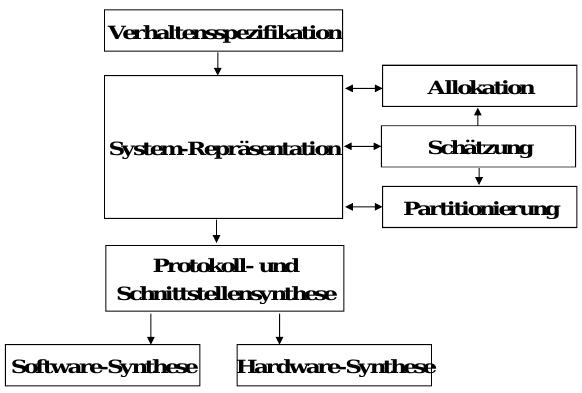
\includegraphics[scale=0.6]{pics/entwurfAufSystemebene}
\end{figure}

\f{Architektursynthese}

\noindent Aufgabe der Architektursynthese: eine strukturelle Sicht aus einer Verhaltensbeschreibung (\zb VHDL) zu generieren. $\Rightarrow$ Grad der Parallelität
\vspace*{5pt}

\ku{wesentlichste Aufgaben}:
\begin{itemize}
 \item Identifikation von Hardware-Elementen, die die spezifizierten Operationen ausführen können (Allokation)
 \item Ablaufplanung zur Bestimmung der Zeitpunkte, an denen die Operationen ausgeführt werden
 \item Binding, d.h. Zuordnung von 
 \begin{itemize}
  \item Variablen zu Speichern 
  \item Operationen zu funktionalen Einheiten
  \item Kommunikationskanäle zu Bussen
 \end{itemize}
\end{itemize}
\f{Modulsynthese}, \f{Logiksynthese}, \f{Blocksynthese}: werden in anderen Vorlesungen genauer behandelt

\section*{Chapter 1.2}
Formale Methoden zur Spezifikation von Systemen sind notwendig, um Realisierungen mit korrektem Verhalten synthetisieren zu können. Spezifizieren mit formalen 
Methoden ist nicht trivial... aber der einzige gehbare Weg!
\vspace*{3pt}

\f{Petri-Netze}
\vspace*{3pt}

\noindent \ku{Definition:}
Ein Petri-Netz ist ein 6-Tupel $G = (P,T,F,K,W,M_0)$ mit 
\begin{itemize}
 \item $P = \{p_1, \dots , p_m\}$ \dots die Menge der Plätze oder Stellen.
 \item $T = \{t_1, \dots , t_n\}$ \dots die Menge der Transitionen.
 \item $P \cap T = \varnothing$. Beide Mengen zusammen bilden die Menge der Knoten.
 \item $F \subseteq (P\times T)\cup(T\times P)$ \dots die Menge der Kanten. Auch Flussrelation genannt.
 \item $K:P \rightarrow N \cup \{\infty \}$, die jedem Platz eine Kapazität zuordnet
 \item $W:F \rightarrow N$, die jeder Kante ein Kantengewicht zuordnet.
 \item $M_0:P \rightarrow N_0$ mit $\forall p\in P:M_0(p)\leq K(p)$, die Anfangsmarkierung
\end{itemize}
Petri-Netze sind also gerichtete bipartite Graphen, denen man eine Interpretation im Sinne erreichbarer Markierungen gibt. Gängige Notation:
\begin{figure}[!ht]
 \centering
 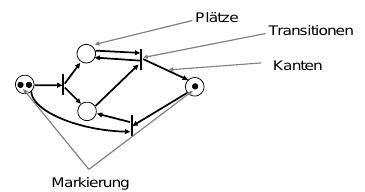
\includegraphics[scale=0.8]{pics/petrinetz}
\end{figure}

\f{Schreibweise}:
\begin{enumerate}
 \item $\forall t\in T:$ \textbullet$t = \{p;(p,t)\in F\}$: Vorbereich von t 
 \item $\forall p\in P:$ \textbullet$p = \{t;(t,p)\in F\}$: Vorbereich von p
 \item $\forall t\in T: t$\textbullet\ $ = \{p;(p,t)\in F\}$: Nachbereich von t 
 \item $\forall p\in P: p$\textbullet\ $ = \{t;(t,p)\in F\}$: Nachbereich von p
\end{enumerate}
\newpage

\f{Schaltbereitschaft von Transitionen}:
\begin{figure}[!ht]
 \centering
 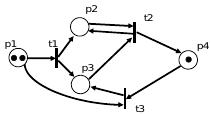
\includegraphics{pics/schaltbereitPetrinetz}
 \caption{Transitionen t1 und t3 sind schaltbereit}
\end{figure}

\noindent Eine Transition $t\in T$ eines Petri-Netzes schaltet von der Markierung $M$ auf $M'$: \[M[t>M'\]
\vspace*{5pt}

\f{Aktivierbare und lebendige Transitionen}
\vspace*{3pt}

\f{Definition}: \ku{Ist $M:P\rightarrow N_0$ eine Markierung eines Petri-Netzes, so heißt eine Markierung $M'$ des Petri-Netzes \f{erreichbar}, wenn}
\begin{itemize}
 \item $\exists t\in T:M[t>M'$
 \item $\exists t\in T:M''[t>M'$ und $M''$ ist von $M$ aus erreichbar
\end{itemize}
$[M>$ bezeichne die Menge der von M aus erreichbaren Markierungen.
\vspace*{6pt}

\noindent Eine Transition $t$ eines Petri-Netzes heißt bzgl. einer Markierung $M$ \f{tot}, wenn sie unter keiner von $M$ aus erreichbaren Markierung schaltbereit ist, 
d.h. $\forall M'\in [M>:\neg(M'[t>)$. Ansonsten heißt sie \f{aktivierbar}.
\vspace*{6pt}

\noindent Eine Transition $t$ eines Petri-Netzes heißt bzgl. einer Markierung $M$ \f{lebendig}, wenn sie bzgl. jeder von $M$ aus erreichbaren Markierung aktivierbar ist.
\vspace*{6pt}

\noindent Ein Petri-Netz heißt \f{deadlockfrei} oder \f{schwach lebendig}, wenn es zu jeder von $M_0$ aus erreichbaren Markierung $M'$ eine Transition $t\in T$ 
gibt, die schaltbereit ist.
\vspace*{6pt}

\noindent Ein Petri-Netz heißt \f{lebendig} oder \f{stark lebendig}, wenn jede seiner Transitionen bzgl. $M_0$ lebendig ist. 
\vspace*{6pt}

\noindent Sei G ein Petri-Netz und $B:P\rightarrow N_0 \cup \{\infty\}$ eine Abbildung, die jeder Stelle eine kritische Markenzahl zuordnet ($B(p)\leq K(p)$). 
Das Petri-Netz G heißt \f{B-sicher} oder \f{B-beschränkt}, wenn $ \forall M\in[M_0>\forall p\in P:M(p)\leq B(p)$.
\vspace*{6pt}

\noindent Das Petri-Netz heißt \f{sicher} oder \f{beschränkt}, wenn es eine natürliche Zahl $b$ gibt, für die G b-beschränkt ist. 
\vspace*{6pt}

\noindent Ein Petri-Netz ist genau dann beschränkt, wenn seine Erreichbarkeitsmenge $[M_0>$ endlich ist.
\vspace*{6pt}

\begin{figure}[!ht]
 \centering
 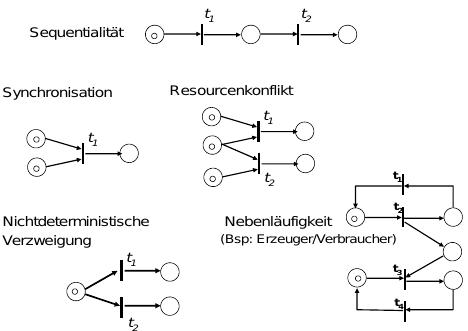
\includegraphics[scale=0.7]{pics/ausdruckPetrinetze}
 \caption{Ausdruckskraft von Petri-Netzen}
\end{figure}

\f{Überdeckung von Markierungen}:
\vspace*{4pt}

\noindent \ku{Annahme}: Die Kapazität eines Platzes ist unendlich. 
\vspace*{4pt}

\noindent Seien $M$ und $M'$ Markierungen. Dann ist $M+M'$ die Markierung, die man durch $M+M'(p) := M(p)+M'(p)$ erhält. Entsprechend sei ``-'' auf Markierungen 
definiert. 
\vspace*{4pt}

\noindent Eine Markierung $M$ \f{überdeckt} $M'(M\geq M')$ genau dann, wenn für alle Plätze $p$ gilt: $M(p)\geq M'(p)$
\vspace*{6pt}

\f{$\omega$-Erweiterungen}
\vspace*{4pt}

\noindent Eine $\omega$-erweiterte Markierung ist gegeben durch $M:P \rightarrow N_0(\omega)$
\vspace*{6pt}

\f{Überdeckungsgraph}
\vspace*{4pt}

\noindent Man kann nun zu jedem Petri-Netz wie folgt einen Überdeckungsgraphen von $M_0$ (ist ein Knoten des Graphen) aus konstruieren:
\begin{itemize}
 \item Knoten: $\omega$-erweiterte Markierungen $M:P\rightarrow N_0 \cup \{\omega \}$
 \item Kanten: Ist $M$ ein Knoten, dann ist für jede feuerbereite Transition $M[t>M'$ 
 
 \qquad \qquad  - $M'$ Nachfolgeknoten, falls kein Vorgänger $M''$ von $M$ existiert mit $M'\geq M''$
 
 \qquad \qquad  - $\Omega(M'',M')$ Nachfolgeknoten, falls $M''$ Vorgänger von $M$ mit $M'\geq M''$
\end{itemize}
\begin{itemize}
 \item Der Überdeckungsgraph ist stets endlich.
 \item Ein Petri-Netz ist beschränkt dann und nur dann, wenn bei der Konstruktion des Überdeckungsgraphen keine $\omega$-erweiterten Knoten entstehen
 \item Petri-Netze können den gleichen Überdeckungsgraphen haben und doch ungleiches Verhalten
 \item Bei beschränkten Petri-Netzen ist das Verhalten genau dann gleich, wenn die Überdeckungsgraphen isomorph sind
\end{itemize}

\begin{figure}[!ht]
 \centering
 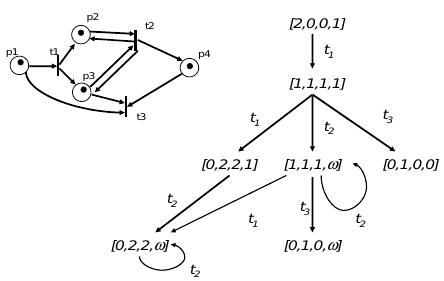
\includegraphics[scale=0.85]{pics/ueberdeckungsgraph}
 \caption{Beispiel für Überdeckungsgraph}
\end{figure}

\f{Zustandsorientierte Modelle}
\vspace*{6pt}

\noindent \f{Definition}: \\ \ku{Ein \f{endlicher} Automat ist gegeben durch ein 6-Tupel $M:=(I,O,S,R,\delta,\lambda)$}. 

\noindent Dabei sind $S,I,O$ endliche Mengen.

\qquad \qquad $S$ heißt \f{Zustandsmenge}, $R \subseteq S$ die Menge der \f{Startzustände} 

\qquad \qquad $I$ heißt \f{Eingabemenge} 

\qquad \qquad $O$ heißt \f{Ausgabemenge} 

\qquad \qquad $\delta:S\times I \rightarrow S$ heißt \f{Übergangsfunktion} 

\qquad \qquad $\lambda:S\times I\rightarrow O$ heißt \f{Ausgabefunktion}

\noindent sind $\lambda$, $\delta$ ``echte'' Relationen, nennt man den Automaten auch \f{nichtdeterministisch}. Sind $\delta$, $\lambda$ partiell, d.h. nicht 
für alle Paare $(s,x)$ definiert, nennt man den Automaten auch unvollständig. 

\noindent Es muss dann aber gelten, dass $\lambda(s,x)$ definiert $\Rightarrow$ $\delta(s,x)$ definiert.

\noindent Endliche Automaten können als Spezialfall interpretierter Petri-Netze aufgefasst werden. Ein nichtdeterministischer endlicher Automat ist ein 
Petri-Netz $G=(P,T,F,K,W,M_0)$ mit 
\begin{itemize}
 \item $\forall t\in T:|$\textbullet$t|=|t$\textbullet$|=1$
 \item $\exists p_0\in P:M_0(p_0) = 1$ und $\forall p\neq p_0:M_0(p) = 0$
 \item $K=W=1$
 \item jeder Transition ist ein Prädikat (Eingabeereignis) als zusätzliche Schaltbedingung und ein Ausgabeereignis als Aktion zugewiesen
\end{itemize}

\f{Statecharts}

\noindent Die Eingabesymbole endlicher Automaten sind in der Regel Sensorsignale oder Zustandssignale kooperierender Automaten. $\Rightarrow$ Notiere die Übergänge als 
Kanten mit Prädikaten (Ereignisse), die auf genau den Eingaben erfüllt sind, unter denen der Übergang stattfindet. 

\noindent Die Ausgabesymbole sind in der Regel Steuersignale für Aktoren. $\Rightarrow$ Notiere neben die Übergangsprädikate Aktionen.

\begin{figure}[!ht]
 \centering
 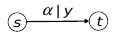
\includegraphics{pics/statechart}
 \caption{Unter allen Eingaben $x$ mit $\alpha(x)$ gehe mit Ausgabe $y$ nach $t$}
\end{figure}

\f{Statecharts -- Gruppierung}:

\noindent Gruppiere Zustände durch Einkreisen und erlaube Übergänge aus Zustandsgruppen. Ein Übergang aus einer Zustandsgruppe steht für Übergänge von jedem Zustand der 
Gruppe aus zu dem gegebenen Zielzustand. 

\begin{figure}[!ht]
 \centering
 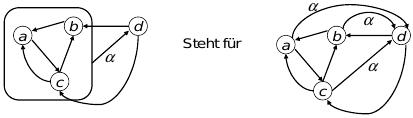
\includegraphics[scale=0.85]{pics/stateUebergang}
\end{figure}

\f{Statecharts -- Hierarchie}:

\noindent Gruppiere Zustände durch Einkreisen, benenne sie und markiere einen Startzustand. 
\begin{figure}[!ht]
 \centering
 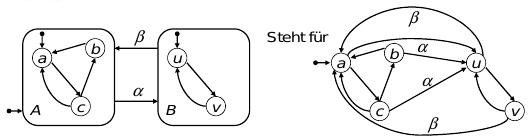
\includegraphics[scale=0.85]{pics/stateHierarchie}
\end{figure}

\f{Statecharts -- Nebenläufigkeit}:

\begin{figure}[!ht]
 \centering
 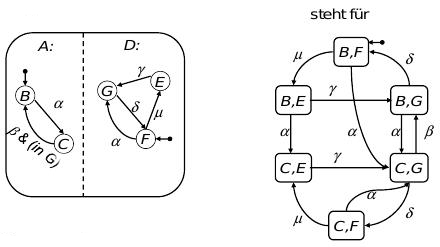
\includegraphics[scale=0.9]{pics/stateNeben}
\end{figure}

\newpage
\f{Datenflussgraphen - DFG}

\noindent DFGs sind gerichtete Graphen, die die durchzuführenden Berechnungen allein über die Verfügbarkeit der dazu notwendigen Daten definieren. Knoten 
entsprechen Operationen (Aktoren), Kanten entsprechen Datenabhängigkeiten. DFGs sind ein Sonderfall von Petri-Netzen: ersetze die Operationsknoten durch 
Transitionen und die Kanten durch Plätze:
\begin{figure}[!ht]
 \centering
 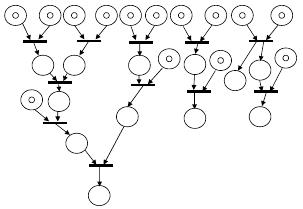
\includegraphics[scale=0.8]{pics/dfgPetri}
\end{figure}

\noindent Jeder Platz hat genau eine Nachfolge- und eine Vorgängertransition, denn jede Datenabhängigkeit hat genau einen Produzenten und genau einen Konsumenten
$\Rightarrow$ markierte Graphen 
\vspace*{6pt}

\f{Markierte Graphen}

\noindent \f{Definition}: \ku{Ein markierter Graph (MG) ist ein Petri-Netz $G=(P,T,F,K,W,M_0)$ mit folgenden Eigenschaften}:
\begin{itemize}
 \item $\forall p\in P: |$\textbullet$p| = |p$\textbullet$| = 1$
 \item $W=1$
 \item $\forall p\in P:K(p)=\infty$
\end{itemize}

\noindent Marken jeder Stelle $p$ werden in der Reihenfolge entnommen, in der sie dort entstehen (FIFO) $\Rightarrow$ keine Konflikte auf den Transitionen. Da in 
MG die Plätze stets genau einen Vorgänger und einen Nachfolger haben, kann man die Plätze auch als Knoten im Netz weglassen und direkt die Kanten zwischen 
Transitionen betrachten und markieren. 
\begin{figure}[!ht]
 \centering
 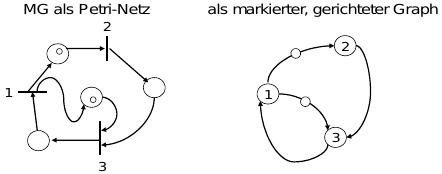
\includegraphics[scale=0.8]{pics/mgpetri}
\end{figure}

Ein Knoten kan feuern, wenn alle einlaufenden Kanten markiert sind. Er nimmt von jeder eingehenden Kante eine Marke und legt auf jede ausgehende Kante eine Marke 
und legt auf jede ausgehende Kante eine Marke. 

\noindent \f{Definition}: Ein markierter Graph ist ein gerichteter Graph $G=(V,E,M_0)$, wobei $M_0:E\rightarrow N_0$ die Anfangsmarkierungen der Kanten ist. 
\vspace*{6pt}

\f{Synchrone Datenflussgraphen}
\vspace*{3pt}

\noindent \f{Definition}: \ku{Ein synchroner Datenflussgraph (SDFG) ist ein Petri-Netz $G=(P,T,F,K,W,M_0)$ mit folgenden Eigenschaften}:
\begin{itemize}
 \item $\forall p\in P: |$\textbullet$p| = |p$\textbullet$| = 1$
 \item $\forall p\in P:K(p)=\infty$
\end{itemize}
\begin{figure}[!ht]
 \centering
 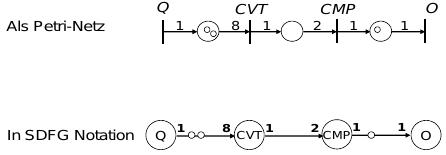
\includegraphics[scale=0.8]{pics/sdfg}
\end{figure}
\newpage
\noindent Marken jeder Stelle $p$ werden in der Reihenfolge entnommen, in der sie dort entstehen (FIFO). Im Unterschied zu markierten Graphen erhalten die Kanten echte 
Gewichte.

\f{Definition}: \ku{Ein SDFG $G$ ist ein 5-Tupel $G=(V,E,cons,prod,d)$ mit }
\begin{itemize}
 \item $V$ ist die Menge der Knoten -- Knoten stehen für Operationen
 \item $E\subseteq V\times V$ ist die Menge der Kanten -- aus Kanten können mehrere Daten liegen. Es gilt FIFO.
 \item $cons:E\rightarrow N$ gibt die Anzahl der beim Feuern des Zielknotens konsumierten Marken an -- sie stehen am Pfeilende
 \item $prod:E\rightarrow N$ gibt die Anzahl der beim Feuern des Quellknotens produzierten Marken an -- sie stehen am Pfeilanfang
 \item $d:E\rightarrow N_0$ gibt die Anfangsmarkierung der Kanten an, d.h. die Anzahl der anfangs auf jeder Kante verfügbaren Daten. 
\end{itemize}

\f{Topologiematrix des SDFG}

\noindent \f{Definition}: \ku{Sei $G=(V,E,cons,prod,d)$ ein SDFG. Die zu $G$ zugehörige Topologiematrix ist ein Matrix $C$ aus $Z^{|V|\times|E|}$, deren Zeilen 
den Knoten und deren Spalten den Kanten von $G$ entsprechen.} Verläuft die Kante $e_j$ vom Knoten $v_i$ zum Knoten $v_k$, so gilt 
\[C[i,j] := -prod(v_i,v_k)\]
\[C[k,j] := cons(v_i,v_k)\]
\[C[l,k] = 0 \text{ für } l\notin\{i,k\}\]
\begin{figure}[!ht]
 \centering
 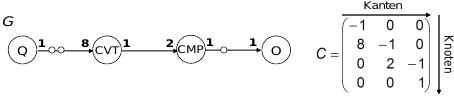
\includegraphics[scale=0.8]{pics/topologie}
\end{figure}

\noindent Ist $d_1$ die momentane Kantenmarkierung und feuert Knoten $v_i$ jeweils $y_i$-mal, so erhält man als resultierende Knotenmarkierung \[d_2 = d_1-C^T y\]
\vspace*{1pt}

\f{Definition}: \ku{Ein zusammenhängender SDFG $G$ mit Topologiematrix $C$ aus $Z^{|V|\times|E|}$ heißt konsistent, wenn die Startmarkierung in endlich vielen 
Schritten wieder angenommen werden kann, d.h. es ein periodisches Verhalten von $G$ gibt.}
\vspace*{4pt}

\noindent \f{Satz}: \ku{Ist $G$ zusammenhängend und konsistent, dann gilt $Rang(C) = |V|-1$}
\vspace*{3pt}

\f{Minimaler Repititionsvektor}
\vspace*{3pt}

\f{Definition}: \ku{Sei $G$ ein zusammenhängender, konsistenter SDFG. Dann heißt der kleinste positive Vektor $y \neq 0$ im Nullraum von $C^T$, d.h.}
\[y\in \{x\in N^{|V|}; C^Tx=0\} \sum_i y_i \text{ minimal}\] \ku{\f{minimaler Repititionsvektor} (von $G$).}
\begin{figure}[!ht]
 \centering
 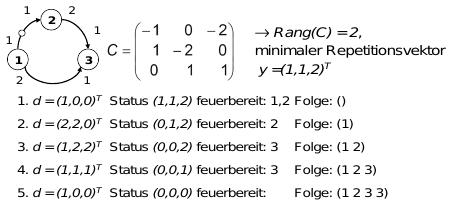
\includegraphics[scale=0.8]{pics/minRepVec}
\end{figure}

\newpage
\f{Verklemmung in SDFG}

\noindent Problem: mit der Existenz eines minimalen Repititionsvektors $y$ ist noch nicht sichergestellt, dass es zu diesem Vektor auch eine konkrete Folge 
schaltbereiter Knoten gibt, so dass jedes $v_i$ genau $y_i$-mal feuert. Das Netz könnte verklemmen. 
\begin{figure}[!ht]
 \centering
 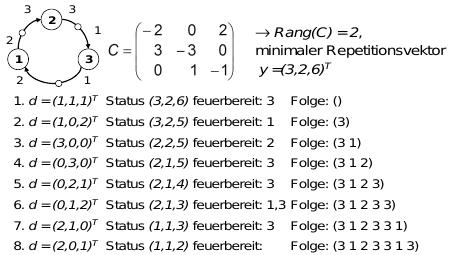
\includegraphics[scale=0.8]{pics/minRepVecVerkl}
 \caption{Beispiel für Verklemmung in einem SDFG}
\end{figure}

\f{Sequenzgraphen}

\noindent \f{Definition}: \ku{Ein Sequenzgraph ist ein azyklischer gerichteter Graph $G=(V,E)$ mit zwei ausgegzeichneten Knoten, einem Start- und einem 
Endknoten. Zusätzlich besitzt $G$ die folgenden Eigenschaften:}
\begin{itemize}
 \item die vom Start- und Endknoten verschiedenen Knoten lassen sich in die folgenden Klassen aufteilen:
 \begin{itemize}
  \item Operationsknoten 
  \item Hierarchieknoten
 \end{itemize}
 \item Hierarchieknoten sind Zeiger auf andere Sequenzgraphen. Man unterscheidet hierbei zwischen dem Modulaufruf (CALL), der Verzweigung (BR) und der Iteration 
 (LOOP) 
\end{itemize}

\section*{Chapter 1.3}
\begin{figure}[!ht]
 \centering
 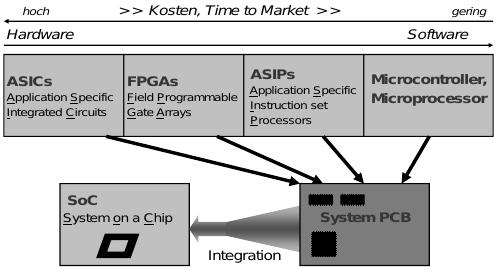
\includegraphics[scale=0.7]{pics/implementierung}
\end{figure}

\f{Allgemeines Synthesemodell}

\noindent \f{Gegeben ist:}
\begin{itemize}
 \item eine Menge von Aufgaben (Operationen, Tasks, \dots), die untereinander Datenabhängigkeiten besitzen können
 \item eine Menge von Ressourcen (ALUs, CPUs, Operatoren, \dots), auf denen jeweils gewisse Aufgaben ablaufen können 
\end{itemize}

\f{Gesucht ist:}
\begin{itemize}
 \item eine Festlegung der Anzahl von Ressourcen $\Leftarrow$ \f{Allokation}
 \item eine Festlegung des zeitlichen Ablaufs der Bearbeitung der Aufgaben unter Berücksichtigung der Datenabhängigkeiten $\Leftarrow$ \f{Ablaufplan (Schedule)}
 \item eine Zuordnung der Aufgaben zu den Ressourcen, so dass zu jeder Zeit jede Ressource höchstens eine Aufgabe bearbeitet $\Leftarrow$ \f{Bindung (Binding)}
\end{itemize}

Je nach Implementierungstechnik werden die Aufgaben unterschiedlich ausgeführt:
\begin{enumerate}
 \item \ku{Allokation}: dieses Problem wird in der Regel beim Entwurf gelöst und hat entscheidenden Einfluss auf die Kosten 
 \item \ku{Ablaufplan}: Ablaufpläne können beim Entwurf gelöst werden (statische Planung) oder zur Laufzeit (dynamische Planung), wobei dynamische Lösungen meist
 bei Softwareimplementierungen, statische eher bei Hardwareimplementierungen genutzt werden 
 \item \ku{Bindung}: Bindungen können ebenso als statische wie dynamische Aufgabe auftreten und von trivial (eine CPU) bis sehr schwierig (mehrere Ressourcen 
 gleichen Typs mit unterschiedlicher Leistung) rangieren
\end{enumerate}

\f{Definitionen}
\begin{itemize}
 \item \f{Sequenzgraph (Problemgraph, Taskgraph)} $G_S=(V,E)$. Sei ein gerichteter azyklischer Graph mit genau einem Start- und genau einem Endknoten. Im 
 folgenden bezeichnen wir mit $V_S\subseteq V$ die Knotenmenge $V$ ohne den Start- und Endknoten und mit $E_S \subseteq E$ die Kanten, die weder den Start- noch 
 den Endknoten als Randknoten besitzen. 
 \item bipartiter \f{Ressourcengraph} $G_R = (V_R, E_R)$ mit $V_R = V_S \cup V_T$ und $E_R \subseteq V_S\times V_T$. $V_T$ ist die Menge der Ressourcentypen 
 (\zb Prozessor, ALU, Addierer, \dots)
 \item \f{Kostenfunktion} $c:V_T\rightarrow N_0$, die die Kosten einer Instanz eines Ressourcentyps angibt 
 \item \f{Ausführungszeiten} $w:E_R\rightarrow N_0$, die jeder Kante $(v_s,v_t)\in E_R$ die Ausführungszeit der Aufgabe $v_S\in V_S$ auf einer Instanz des 
 Ressourcentyps $v_t \in V_T$ angibt
 \item ein \f{Syntheseproblem} $P$ ist gegeben durch ein Tupel $P = (G_S,G_R)$
\end{itemize}

\f{Definition -- Allokation}: \ku{Gegeben sei ein Syntheseproblem. Eine Allokation ist eine Funktion $\alpha:v_T\rightarrow N_0$, die jedem Ressourcentyp 
$v_t\in V_T$ eine Anzahl $\alpha(v_t)$ verfügbarer Instanz zuordnet.}
\vspace*{5pt}

\f{Definition -- Ablaufplan}: \ku{Gegeben sei ein Syntheseproblem. Ein Ablaufplan (Schedule) eines Sequenzgraphen $G_S=(V,E)$ ist eine Funktion 
$\uptau:V_S \rightarrow N_0$, die jedem Knoten $v_S \in V_S$ die Startzeit $\uptau(v_S)$ zuordnet und für jede Kante $(v_s,v_t)\in E_S$ die Bedingung}
\[\uptau(v_t) - \uptau(v_s)\geq w(v_s)\] 
\ku{erfüllt. Hierbei gibt $w(v_s)$ die Laufzeit der Aufgabe $v_s$ auf ihrer Ressource an.}

\f{Definition -- Latenz}: \ku{Die Latenz eines Ablaufplans $\uptau$ eines Sequenzgraphens $G_S = (V,E)$ ist definiert als}
\[L(\uptau) = \text{ späteste Beendungszeit $-$ früheste Startzeit } = max\{\uptau(v_i) + w(v_i); v_i \in V_S\} - min\{\uptau(v_j);v_j\in V_S\}\]

\f{Definition -- Bindung}: \ku{Eine Bindung eines Sequenzgraphens $G_S = (V,E)$ bzgl. eines Ressourcengraphen $G_R = (V_R,E_R)$ und einer Allokation 
$\alpha: V_T \rightarrow N_0$ ist ein Paar von Funktionen $\beta:V_S\rightarrow V_T$ und $\gamma:V_S \rightarrow N$ mit }
\begin{itemize}
 \item $\forall v_s \in V_S:(v_s,\beta(v_s)) \in E_R$
 \item $\forall v_s \in V_S:\gamma(v_s)\leq \alpha(\beta(v_s))$
\end{itemize}

\ku{d.h. die Bindung ordnet jeder Aufgabe eine verfügbare Instanz einer Ressource zu, die diese Aufgabe ausführen kann.}
Liegt ein Ablaufplan vor, so muss ferner gelten, dass zu jedem Zeitpunkt $t$ jeder Ressource nur eine Aufgabe zugeordnet ist.
\end{chapter}

\begin{chapter}{Kapitel}
 \section*{Chapter 2.1}
 
 \f{Verifikation}: \ku{check that we are building the thing right}
 \vspace*{3pt}
 
 \noindent Soll den Nachweis liefern, dass das System die Anforderungen immer erfüllt (Korrektheit der Implementierung in Bezug auf die Spezifikation).
 \vspace*{3pt}
 
 \f{Validation}: \ku{check that we are building the right thing}
 \vspace*{3pt}
 
 \noindent Entspricht eher dem kritischen Überprüfen der Spezifikation anhand eines ersten Designs auf Richtigkeit und Vollständigkeit.
 
 \f{Testen}: \ku{ist ein Mittel für beides und weit verbreitet.}
 \vspace*{3pt}
 
 \noindent Verifikation lässt sich damit nicht bewerkstelligen, allenfalls Falsifikation. 
 \vspace*{8pt}
 
 \f{Populäre Techniken der Verifikation}:
\begin{itemize}
 \item \f{Peer Reviewing}: Statische Methode der manuellen Durchsicht und Prüfung des Codes durch einen Experten. Im Mittel bringt dies 60\% der Fehler, subtile
 Fehler werden meist nicht gefunden.
 \item \f{Testen}: Dynamische Methode, häufig unterstützt durch Qualitätsmetriken (Code Coverage). 30\% bis 50\% der Gesamtkosten gehen auf das Konto von Testen, 
 bei Hardware sind oft 70\% des entwickelten Codes Testbenches.
\end{itemize}
Man kann mit Tests die Anwesenheit von Fehlern nachweisen, nicht jedoch deren Abwesenheit!
\vspace*{8pt}

\f{Formale Methoden}:
\vspace*{4pt}

\noindent Formale Methoden basieren auf formalen Sprachen zur Spezifikation von Eigenschaften wie auch zur Konstruktion des Systems. Gebräuchliche 
Verifikationstechniken mit formalen Methoden sind:
\begin{itemize}
 \item \f{Deduktive Methoden}: Hier liefert man einen mathematischen Beweis, dass die Implementierung die Spezifikation erfüllt. Meist werden Theorembeweiser 
 oder Beweisprüfer als Werkzeuge benutzt. Problem: Sehr aufwändig, das System muss die Form einer Mathematischen Theorie haben.
 \item \f{Model Checking}: Systematische und erschöpfende Überprüfung der Spezifikation auf allen erreichbaren Systemzuständen. Meist vollautomatisch durch 
 sogenannte Modellchecker. Problem: Zustandsraumexplosion
 \item \f{Modelbasierte Simulation und Test}: Exploration möglicher Verhalten mit Überprüfung der Spezifikationen
\end{itemize}

\f{Model-Checking}:
\vspace*{4pt}

\noindent Man betrachtet 
\begin{itemize}
 \item \f{Spezifikation}: formale Definition der Eigenschaften des gewünschten Systems in Form von Sätzen einer mathematischen Theorie (Aussagen einer temporalen 
 Logik)
 \item \f{Implementierung}: formale Definition der konkreten Konstruktion des Systems (als diskretes Transitionssystem)
 \item \f{Model Checking}: Ist die Implementierung ein Modell für die Theorie (gelten die Sätze für die Implementierung)
\end{itemize}
\begin{figure}[!ht]
 \centering
 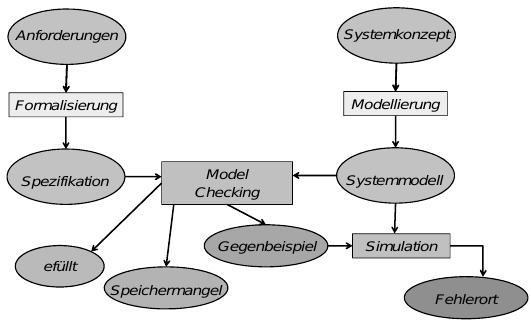
\includegraphics[scale=0.8]{pics/modelchecking}
\end{figure}

\f{Transitionssysteme}:

\f{Definition}: \ku{Ein Tupel $T=(S,(Act,)\rightarrow, St)$ heißt Transitionssystem, wobei}
\begin{itemize}
 \item $S$ \dots eine Menge von Zuständen 
 \item $\rightarrow \subseteq S\times S$ die Transitionsrelation ($\rightarrow \subseteq S\times Act \times S$)
 \item $Act$ eine Menge von Aktionen 
 \item $St \subseteq S$ eine Menge von Startzuständen ist 
\end{itemize}

\noindent Auf die Startzustände kann man auch verzichten oder auf genau einen gehen, der dann vermöge $\rightarrow$ nichtdeterministisch in $St$ verzweigt.
\vspace*{4pt}

\noindent Auch die Aktionen sind Komfort, sie machen es leichter, mehrere kooperierende Transitionssysteme zu definieren und Synchronisationsbedingungen über Aktionen zu 
formulieren. Wenn wir die Zustandsmenge endlich machen und die Aktionen als Ein/Ausgabemarkierungen auffassen, sind wir wieder bei unseren vertrauten Automaten.
\vspace*{4pt}

\noindent Bei endlicher Zustandsmenge ist auch klar, dass man die Übergangsrelation als gerichteten Graphen darstellen kann. 
\begin{figure}[!ht]
 \centering
 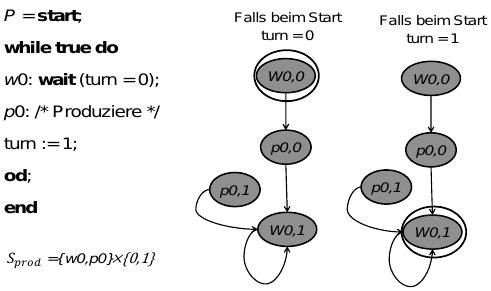
\includegraphics[scale=0.8]{pics/transitionssystem}
 \caption{Producer als Transitionssystem}
\end{figure}

\f{Kripke-Strukturen}:
\vspace*{4pt}

\noindent Praktisch stellt man Eigenschaften eines Systems durch Messung fest, d.h. Eigenschaften sind im einfachsten Falle binär, sie gelten oder gelten nicht.
\vspace*{4pt}

\noindent Alles was wir über das Verhalten eines System wissen oder erfahren können sollte sich also grundsätzlich gesehen auf endlich viele (wir können nur endlich viel 
messen) \f{atomare Aussagen} zurückführen lassen. Wir erweitern ein Transitionssystem zu einer \f{Kripke Struktur}: 

\[K = (S,(Act,)\rightarrow, St, AP, L)\]

\noindent Dabei kommen noch zwei Komponenten dazu: 
\begin{itemize}
 \item $AP$ \dots eine (endliche) Menge von atomaren Aussagen (atomic propositions)
 \item $L:S \rightarrow 2^{AP}$ \dots eine Markierung der Zustände mit den durch sie erfüllten atomaren Aussagen (labeling) 
\end{itemize}

\newpage 
\noindent Das Transitionssystem zu den Producer/Consumer-Prozessen könnte man durch folgende atomare Aussagen erweitern: \[AP=\{p,k\}\] mit $p$: es wird gerade produziert 
\\ und $k$: es wird gerade konsumiert
\vspace*{5pt}

\f{Linear-Zeit vs. Baum-Zeit}:
\vspace*{5pt}

\noindent Formal werden wir zu verifizierende Eigenschaften unserer Systeme in \f{temporaler Logik} ausdrücken. 
\vspace*{4pt}

\noindent Die \f{Linear-Zeit Logik (linear time logic, LTL)} erlaubt Aussagen über Labelings aller (unendlichen) Berechnungsfolgen der Kripke-Struktur. 
LTL-Aussagen gelten entweder für alle Folgen oder nicht. 
\vspace*{4pt}

\noindent Die \f{Baum-Zeit Logik (computation tree logic, CTL)} erlaubt die Formulierung von Aussagen über Berechnungsbäume, d.h. man kann Existenz und 
Allquantoren für die Pfade in den Unterbäumen nutzen.

\section*{Chapter 2.2}
\f{Linear-Time Logic} 
\vspace*{3pt}

\noindent Linear-Zeit Logik ist eine Logik, die auf Sequenzen von Belegungen mit atomaren Eigenschaften basiert. Die Zeit ist diskret und schreitet linear voran. Es gibt 
nur eine mögliche Zukunft.
\vspace*{4pt}

\noindent Sei $AP$ die Menge der atomaren Aussagen. Dann korrespondiert das Labeling $X \subseteq AP$ zu der Tatsache, dass alle Eigenschaften $x\in X$ in dem 
Zustand gelten und alle $y\in AP\setminus X$ in diesem Zustand nicht gelten.

\noindent LTL Formeln werden nun über Mengen von unendlichen Folgen von Labelings interpretiert. D.h. wir betrachten Sequenzen $\sigma \in (2^{AP})^\omega$, wofür
ein Alphabet $\Sigma, \Sigma^\omega$ die Menge aller unendlichen Folgen über $\Sigma$ sei. 

\noindent Für $\sigma \in (2^{AP})^\omega$ sei 
\begin{itemize}
 \item $\sigma(i) \subseteq AP$ das i-te Element der Folge
 \item $\sigma^i \in (2^{AP})^\omega$ die unendliche Folge $\sigma(i)\sigma(i+1)\sigma(i+2)\dots$
\end{itemize}
\vspace*{5pt}

\f{Syntax von LTL}:
\vspace*{4pt}

\noindent Sei $AP$ eine Menge von atomaren Aussagen. Dann ist die Menge der LTL Formeln über $AP$ wie folgt definiert: 
\begin{enumerate}
 \item jedes $p\in AP$ ist eine LTL Formel 
 \item sind $\Phi_1$ und $\Phi_2$ Formeln, dann auch $\neg \Phi_1$, $\Phi_1 \vee \Phi_2$, $\f{X}\Phi_1$, $\Phi_1\f{U}\Phi_2$
 \item nichts sonst ist eine LTL Formel 
\end{enumerate}

\noindent Dies ist eine sehr minimalistische Definition. \f{X} (next) und \f{U} (until) sind temporale Operatoren. 
\vspace*{4pt}

\noindent LTL Formeln werden über (unendlichen) Folgen von Teilmengen atomarer Aussagen interpretiert. Die Semantik einer LTL-Formel $\Phi$ ist die Menge aller 
Folgen $\sigma \in (2^{AP})^\omega$, die $\Phi$ erfüllen, d.h. 
\[[[\Phi]] = \{\sigma | \sigma \vDash \Phi\}\]

\f{Erfüllung einer LTL-Formel}:
\vspace*{5pt}

\noindent Sei $\sigma \in (2^{AP})^\omega$ und sei $\Phi$ eine LTL Formel. Dann gilt $\sigma \vDash \Phi$ (``$\sigma$ erfüllt $\Phi$'') nach folgender
Fallunterscheidung über die Struktur von $\Phi$:
\begin{itemize}
 \item $\sigma \vDash p$ \qquad \qquad   falls $p\in AP$ und $p\in\sigma(0)$
 \item $\sigma \vDash \neg\Phi$ \qquad  \qquad falls $\sigma \nvDash \Phi$
 \item $\sigma \vDash \Phi_1 \vee \Phi_2$ \qquad falls $\sigma \vDash \Phi_1$ oder $\sigma \vDash \Phi_2$
 \item $\sigma \vDash \f{X}\Phi$ \qquad  \qquad falls $\sigma^1 \vDash \Phi $
 \item $\sigma \vDash \Phi_1\f{U}\Phi_2$ \qquad falls $\exists i: \left(\sigma^i\vDash \Phi_2 \wedge \forall k < i:\sigma^k \vDash \Phi_1 \right)$
\end{itemize}
\vspace*{5pt}

\f{Nützliche Abkürzungen für LTL-Formeln}:
\vspace*{4pt}

\f{F} \dots finally (``irgendwann''), \f{G} \dots globally (``immer''), \f{W} \dots weak until, \f{R} \dots releases
\begin{itemize}
 \item $\Phi_1\wedge\Phi_2 \equiv \neg(\neg\Phi_1\vee\neg\Phi_2)$
 \item $\Phi_1 \rightarrow \Phi_2 \equiv \neg\Phi_1\vee\Phi_2$
 \item $true \equiv a\vee\neg a$
 \item $false \equiv \neg true$
 \item $\f{F}\Phi \equiv true\f{U}\Phi$
 \item $\f{G}\Phi \equiv \neg\f{F}\neg\Phi$
 \item $\Phi_1\f{W}\Phi_2 \equiv (\Phi_1\f{U}\Phi_2)\vee\f{G}\Phi_1$
 \item $\Phi_1\f{R}\Phi_2 \equiv \neg(\neg\Phi_1\f{U}\neg\Phi_2)$
\end{itemize}
\vspace*{5pt}

\f{Tautologie, Unerfüllbarkeit, Äquivalenz}:
\vspace*{4pt}

\f{Tautologie}: Jede Formel $\Phi$ mit $[[\Phi]] = \left(2^{AP}\right)^\omega$ heißt Tautologie
\vspace*{4pt}

\f{Unerfüllbarkeit}: Jede Formel $\Phi$ mit $[[\Phi]] = \varnothing$ heißt unerfüllbar
\vspace*{4pt}

\f{Äquivalenz}: zwei Formeln $\Phi_1$ und $\Phi_2$ heißen äquivalent, gdw. $[[\Phi_1]] = [[\Phi_2]]$. Wir schreiben dann auch $\Phi_1 \equiv \Phi_2$
\vspace*{6pt}

\f{Idempotenz und Rekursionsgesetze}:
\vspace*{5pt}

\begin{itemize}
 \item $\f{F}\Phi \equiv \f{FF}\Phi$
 \item $\f{G}\Phi \equiv \f{GG}\Phi$
 \item $\Phi\f{U}\Psi \equiv \Phi\f{U}(\Phi\f{U}\Psi)$
 \item Rekursionsgesetze:
 \begin{itemize}
  \item $\f{F}\Phi \equiv \Phi\vee\f{XF}\Phi$
  \item $\f{G}\Phi \equiv \Phi\wedge\f{XG}\Phi$
  \item $\Phi\f{U}\Psi \equiv \Psi\vee(\Phi\wedge\f{X}(\Phi\f{U}\Psi))$
  \item $\Phi\f{W}\Psi \equiv \Psi\vee(\Phi\wedge\f{X}(\Phi\f{W}\Psi))$
 \end{itemize}
\end{itemize}
\vspace*{5pt}

\f{Sicherheitseigenschaften}:
\vspace*{4pt}

\noindent Eine Eigenschaft ist eine Sprache $L \subseteq \left(2^{AP}\right)^\omega$. Gibt es für alle $\sigma \in \left(2^{AP}\right)^\omega/L$ einen endlichen Präfix $w$,
so dass für alle $\alpha \in \left(2^{AP}\right)^\omega$ schon gilt $w\alpha \notin L$, d.h. es gibt keine zulässige Erweiterung mehr, mit der man den Präfix $w$
wieder nach $L$ bringen kann, dann nennt man $w$ einen \f{schlechten Präfix} und $L$ eine \f{Sicherheitseigenschaft}.
\vspace*{6pt}

\f{Lebendigkeitseigenschaften}:
\vspace*{4pt}

\noindent Es gilt $L \subseteq \left(2^{AP}\right)^\omega$. Gibt es für jedes $w \in \left(2^{AP}\right)^*$ ein $\alpha \in \left(2^{AP}\right)^\omega$ so dass 
wieder $w\alpha \in L$, d.h. es gibt stets eine zulässige Erweiterung, mit der man einen Präfix $w$ nach $L$ bringen kann, dann nennt man $L$ eine 
\f{Lebendigkeitseigenschaft}.
\vspace*{5pt}

\noindent Jede LTL-Eigenschaft lässt sich als Schnitt einer Sicherheitseigenschaft mit einer Lebendigkeitseigenschaft darstellen. 
\vspace*{4pt}

\f{Interpretation von LTL über Kripke-Strukturen  }
\vspace*{5pt}

\noindent Kripke Strukturen sind ja die formalen Modelle, die wir für Implementierungen von Systemen betrachten. Wenn wir nun wissen wollen, ob ein System in LTL 
formulierte Eigenschaften erfüllt, müssen wir nachprüfen, ob die Eigenschaft über den Menge aller (unendlichen) Ausführungsfolgen der Kripke Struktur gilt. 
\vspace*{4pt}

\noindent Sei $K = (S,\rightarrow, St, AP,L)$ eine Kripke-Struktur. 
\vspace*{4pt}

\noindent Eine Folge $\rho \in S^\omega$ mit $\rho(1)\in St$ und $\forall i:\rho(i)\rightarrow \rho(i+1)$ heißt Ausführung von $K$.
\vspace*{4pt}

\noindent Für eine Ausführung $\rho$ betrachten wir nun  $L(\rho) \in \left(2^{AP}\right)^\omega$ mit $\forall i: L(\rho)(i):=L(\rho(i))$, d.h. die 
Labelingfolge zur Ausführung $\rho$. 
\vspace*{4pt}

\noindent Dann bezeichnen wir mit $[[K]]$ die Menge aller möglichen Labelingsequenzen zu Ausführungen von K. 
\vspace*{4pt}

\[[[K]] = \{L(\rho)|\rho \text{ ist Ausführung von } K \}\]

\f{Das LTL-Model-Checking Problem}
\vspace*{4pt}

\noindent Das Problem ist es, zu entscheiden, ob eine Kripke Struktur, die wir aus der Implementierung abgeleitet haben, ein Modell für die Spezifikation ist. 
\vspace*{4pt}

\noindent Gegeben sei eine Kripke-Struktur $K=(S,\rightarrow, St,AP,L)$ und eine LTL-Formel $\Phi$ über $AP$. Entscheide, ob $[[K]] \subseteq [[\Phi]]$.
\vspace*{4pt} 

\noindent Es muss also für jede Ausführung $\rho$ das Labeling $L(\rho)$ die Formel $\Phi$ erfüllen. Wir schreiben dann auch $K \vDash \Phi$.

\noindent Vorsicht: es kann sowohl $K \vDash \Phi$ als auch $K \nvDash \neg\Phi$ gelten!
\vspace*{6pt}

\f{Fallstrick endliche Ausführungen}:
\vspace*{4pt}

\noindent Vorsicht: LTL Formeln werden nur über den unendlichen Ausführungen interpretiert.
\vspace*{4pt}

\noindent Wenn die Kripke Struktur zum Beispiel Deadlocks enthält (Zustände ohne Nachfolger in der Transitionsrelation), dann werden alle Ausführungen, die auf 
einem solchen Zustand enden ignoriert, weil sie endliche Länge haben. Auf solchen Ausführungen wird die Formel nicht interpretiert.
\vspace*{4pt}

\noindent Das kann im Extremfall unerwartete Konsequenzen haben: Angenommen in $K$ führt jeder Weg in einen Deadlock. Dann ist $[[K]] = \varnothing$. Damit 
erfüllt $K$ aber jede Formel!
\vspace*{6pt}

\f{LTL-Model-Checking}
\vspace*{4pt}

\noindent Wir wollen nun anschauen, wie man (im Prinzip, schnelle Heuristiken sind nach wie vor Gegenstand der aktuellen Forschung) Model Checking für LTL Formeln 
algorithmisch entscheidet:

\noindent Gegeben sei eine Kripke-Struktur $K=(S,\rightarrow, St,AP,L)$ und eine LTL-Formel $\Phi$ über $AP$. Entscheide, ob $[[K]] \subseteq [[\Phi]]$.

\noindent Im Prinzip gibt es zwei Möglichkeiten: 
\begin{enumerate}
 \item Konstruiere eine LTL-Formel $\Psi$ mit $[[K]] = [[\Psi]]$ und zeige $\Psi \rightarrow \Phi$. Dies ist sehr aufwändig.
 \item Die Menge der Ausführungen von $K$ lässt sich leicht als Sprache eines Büchi Automaten $BA(K)$ d.h. $[[K]] = L(BA(K))$ auffassen. Konstruiere einen weiteren 
 Büchi Automaten $BA(\neg \Phi)$ der die Sprache $[[\neg\Phi]]$ akzeptiert und entscheide \[L(BA(K)) \cap L(BA(\neg\Phi)) = \varnothing\]
\end{enumerate}

\f{Büchi-Automaten}
\vspace*{4pt}

\noindent Büchi-Automaten sind im Prinzip endliche Automaten mit einem anderen Akzeptanzkriterium. Ein Tupel $B=(S,S_0,A,\Delta,F)$ heißt \f{Büchi-Automat}, 
wobei
\begin{itemize}
 \item $S$ \dots eine endliche Menge von Zuständen 
 \item $S_0 \subseteq S$ eine Menge von Startzuständen 
 \item $\Delta \subseteq S\times A \times S$ die Übergangsrelation
 \item $A$ ein endliches Alphabet
 \item $F \subseteq S$ eine Menge von Endzuständen (Akzeptanzzuständen) ist.
\end{itemize}
Man kann Büchi Automaten ebenso durch Diagramme darstellen, wie man das von endlichen Automaten kennt lediglich die Sprache ist anders definiert:

\noindent Sei $B=(S,S_0,A,\Delta,F)$ ein Büchi-Automat. 

\noindent Für ein unendliches Wort $\sigma \in A^\omega$ ist $s(1)\sigma(1)s(2)\sigma(2)\dots s(i)\sigma(i)\dots$ ein Lauf in $B$ mit Beschriftung $\sigma$ 
genau dann wenn
\begin{itemize}
 \item $s(1) \in S_0$ und
 \item für alle $i$ gilt $s(i)\sigma(i)s(i+1)\in \Delta$
\end{itemize}
Ein Lauf heißt akzeptierend, wenn für unendlich viele $i$ gilt: $s(i)\in F$. 

Ein Büchi-Automat $B = (S,S_0,A,\Delta,F)$ akzeptiert die Sprache $L(B) \subseteq A^\omega$ genau dann, wenn es für jedes $\sigma\in L(B)$ einen akzeptierenden 
Lauf mit Beschriftung $\sigma$ gibt. 
\vspace*{5pt}

\f{Büchi-Automaten und LTL}:
\vspace*{5pt}

\noindent Sei $AP$ wieder eine Menge atomarer Eigenschaften. Setzt man $A = 2^{AP}$, dann sind Worte aus $A^\omega$ wieder unendliche Verhaltensmuster über $AP$. 
\vspace*{5pt}

\noindent Wir werden sehen, dass man zu jeder LTL Formel $\Phi$ über $AP$ einen Büchi Automaten $BA(\Phi)$ angeben kann, mit $L(BA(\Phi)) = [[\Phi]]$ d.h. der nur
Läufe akzeptiert auf denen die Formel gilt. Zeigen tun wir das zunächst an einem Beispiel:
\vspace*{5pt}

\noindent Für die Formel $G(p \rightarrow Fq)$ über $AP=\{p,q\}$ akzeptiert folgender Automat die Sprache $[[G(p\rightarrow Fq)]]$
\begin{figure}[!ht]
 \centering
 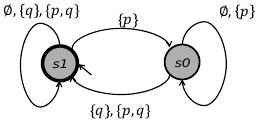
\includegraphics{pics/automatpq}
\end{figure}

\f{Der Produktautomat}
\vspace*{5pt}

\noindent Gegeben seien zwei Büchi-Automaten $B_1=(S_1,S_{1,0},A,\Delta_1,F_1)$, $B_2=(S_2,S_{2,0},A,\Delta_2,F_2)$ als Akzeptoren zweier $\omega$ regulärer
Sprachen $L(B_1),L(B_2)$:  \\ wir definieren den \f{Produktautomaten} $B_{1\times2} =(S_{1\times2},S_{1\times2,0},A,\Delta_{1\times2},F_{1\times2})$ durch 
\begin{itemize}
 \item $S_{1\times2} := S_1\times S_2$
 \item $S_{1\times2,0} := S_{1,0}\times S_{2,0}$
 \item $\Delta_{1\times2} := \{((s_1,s_2),a,(t_1,t_2))|(s_1,a,t_1)\in \Delta_1 \wedge (s_2,a,t_2)\in \Delta_2\}$
 \item $F_{1\times2} := F_1\times F_2$
\end{itemize}
\vspace*{6pt}
\f{LTL-Model-Checking}
\vspace*{5pt}

\noindent Wir haben nun eine Möglichkeit entwickelt, mit der man (im Prinzip, schnelle Heuristiken sind nach wie vor Gegenstand der aktuellen Forschung) Model 
Checking für LTL Formeln algorithmisch durchführen kann:

\noindent Gegeben sei eine Kripke-Struktur $K=(S,\rightarrow, St,AP,L)$ und eine LTL-Formel $\Phi$ über $AP$. Entscheide, ob $[[K]] \subseteq [[\Phi]]$.
\begin{enumerate}
 \item die Kripke Struktur $K$ stammt in der Regel von einer Spezifikation des Systems in Form eines Automaten. Bei unendlichem Betrieb lässt sich diese leicht 
 durch einen Büchi-Automaten $BA(K)$ ausdrücken. 
 \item übersetze die LTL Formel $\Phi$ in einen Büchi-Automaten $BA(\neg\Phi)$ der die Sprache $[[\Phi]]$ akzeptiert.
 \item bilde den Produktautomaten $BA(L(BA(K)))\cap L(BA(\neg\Phi))$ und entscheide, ob  die Menge der akzeptierenden Läufe leer ist. 
 \item gibt es einen akzeptierenden Lauf, ist dieser ein Gegenbeispiel.
\end{enumerate}

\section*{Chapter 2.3}
\f{Baum-Zeit-Logik}

\noindent Linear-Zeit Logik ist eine Logik, die sich auf alle unendlichen Sequenzen von Belegungen mit atomaren Eigenschaften bezieht. Es gibt nur eine 
mögliche Zukunft. Man kann nicht über alternative Möglichkeiten den Entwicklung Aussagen machen. Baum-Zeit Logik erlaubt Aussagen über die Möglichkeiten eines
Systems. Prominentester Vertreter ist CTL (Computation Tree Logic).
\vspace*{5pt}

\noindent Beispiel (siehe Bild): $\Rightarrow$ lässt sich nicht in LTL adäquat beschreiben. Es gibt sowohl Folgen, in denen $p$ nie gilt, als auch Folgen, in denen $p$ 
irgendwann mal gilt. 

\begin{figure}[!ht]
 \centering
 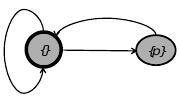
\includegraphics{pics/ctl}
\end{figure}

\f{Belegungsbaum zu einer Kripke-Struktur}:
\vspace*{4pt}

\noindent Sei $K=(S,\rightarrow,s_0,AP,L)$ eine Kripke-Struktur mit Startzustand $s_0$. Für $s\in S$ sei ein Belegungsbaum $T_K(s)$ zu $K$ mit Wurzel $s$ wie folgt
definiert: 
\vspace*{4pt}

\noindent Zu jedem $s'\in S$ mit $s\rightarrow s'$ gibt es genau einen zu $T_K(s')$ isomorphen Unterbaum von $T_K(s)$. 
\vspace*{4pt}

\noindent $T_K(s)$ beschreibt quasi eine Entfaltung der Kripke-Struktur in einen unendlich tiefen Baum. 
\vspace*{5pt}

\noindent CTL-Formeln werden über Berechnungsbäume interpretiert. Sie machen bei jedem temporalen Operator eine Aussage über die Menge der möglichen 
Entwicklungen im Baum durch existenzielle oder universelle Quantifizierung.
\vspace*{5pt}

\f{Syntax von CTL}:
\vspace*{4pt}

\noindent Sei $AP$ eine Menge von atomaren Aussagen. Dann ist die Menge der CTL-Formeln über $AP$ wie folgt definiert: 
\begin{itemize}
 \item jedes $p\in AP$ ist eine CTL-Formel
 \item sind $\Phi_1$ und $\Phi_2$ Formeln, dann auch $\neg\Phi_1$, $\Phi_1 \vee\Phi_2$, $\f{EX}\Phi_1$, $\f{EG}\Phi_1$,$\Phi_1\f{EU}\Phi_2$
 \item nichts sonst ist eine CTL-Formel
\end{itemize}
\f{EX} \dots exists next, \f{EG} \dots exists globally und \f{EU} \dots exists until sind temporale Operatoren.

\noindent Alle anderen Operatoren kann man durch Formeln über diese ausdrücken. 
\vspace*{5pt}

\f{Nützliche Abkürzungen für CTL-Formeln}:
\begin{itemize}
 \item $\Phi_1\wedge\Phi_2 \equiv \neg(\neg\Phi_1\vee\neg\Phi_2)$
 \item $true \equiv a\vee\neg a$
 \item $\f{EF}\Phi \equiv true\f{EU}\Phi$
 \item $\f{AX}\Phi \equiv \neg\f{EX}\neg\Phi$
 \item $\f{AF}\Phi \equiv \neg\f{EG}\neg\Phi$
 \item $\Phi_1\f{AU}\Phi_2 \equiv \f{AF}\Phi_2 \wedge (\Phi_1\f{AW}\Phi_2)$
 \item $\Phi_1 \rightarrow \Phi_2 \equiv \neg\Phi_1\vee\Phi_2$
 \item $false \equiv \neg true$
 \item $\Phi_1\f{EW}\Phi_2 \equiv (\Phi_1\f{EU}\Phi_2)\vee\f{EG}\Phi_1$
 \item $\f{AG}\Phi \equiv \neg\f{EF}\neg\Phi$
 \item $\Phi_1\f{AW}\Phi_2 \equiv \neg(\neg\Phi_2\f{EU}\neg(\Phi_1\vee\Phi_2))$
\end{itemize}ju
\f{A} \dots all (für alle Pfade), \f{F} \dots future, \f{W} \dots weak until
\vspace*{5pt}

\f{Beispiele: siehe Übungsblätter}

\end{chapter}

\begin{chapter}{Ablaufplanung}
  \f{Unterscheidungskriterien}
  \begin{itemize}
   \item statische vs. dynamische -- statische Ablaufpläne treten auf, wenn zur Übersetzungs-/Synthesezeit ein Ablaufplan erstellt werden muss, vor allem bei hardwarenahem Implementationstechnicken. Dynamische Ablaufpläne treten zur Laufzeit des ES auf, meist bei Softwareimplementierungen.
   \item präemptiv vs nicht-präemptiv -- bei präemptiven Plänen geht man davon aus, dass die Laufzeit eines Jobs viel länger ist als die Dauer, ihn zu pausieren, meist Software. Bei kurzen oder nicht-unterbrechbaren Jobs verwendet man nicht-präemptive Pläne.
   \item Abhängigkeitsbedingungen -- bei Datenabhängigkeiten unterliegt der Plan zeitlichen Einschränkungen, gegeben durch DAG. Kommen sehr häufig vor.
   \item Ressourcenbeschränkungen -- Hardware (PUs, Busse, Speicher) als Nebenbedingung, Probleme werden schwerer.
   \item Zeitbeschränkungen -- 
   \begin{itemize}
    \item absolute: Deadlines \& Release-Termine
    \item relative: zeitliche Bedingungen zwischen den einzelnen Jobs (Start- \& Endzeitpunkte)
   \end{itemize}
   \item periodisch vs. aperiodisch -- periodische Probleme kommen bei Iterationen vor, periodische Einplanung. Findet Verwendung bei Schleifenoptimierungen oder DSP.
  \end{itemize}
  
  \begin{section}{Statische Ablaufplanung}
   \begin{subsection}{Statische Ablaufplanung ohne Ressourcenbeschränkungen} 
    ist einfach und kann von gängigen Graph-Algorithmen effizient gelöst werden.
    
   \f{der As Soon as Possible-Algorithmus (ASAP) (Komplexität $O(|V| + |E|)$)}
   \begin{itemize}
    \item berechne topologische Sortierung
    \item verplane jeden Knoten in Reihenfolge der topologischen Sortierung vom frühest möglichen Zeitpunkt (wenn die entsprechende Ressoure wieder frei ist)
   \end{itemize}

   Dieser Algorithmus liefert einen Ablaufplan minimaler Latenz $\rightarrow$ untere Schranke für Pläne mit Zeit- \& Ressourcenbeschränkungen. (Beweisbar über Induktion über die Startzeitpunkte.) 
   
   \f{der As Late as Possible-Algorithmus (ALAP) (Komplexität $O(|V| + |E|)$)}
   \begin{itemize}
    \item berechne umgekehrte topologische Sortierung
    \item verplane jeden Knoten in Reihenfolge der umgekehrten Sortierung vom spätest möglichen Zeitpunkt (beachte kritische Pfade)
   \end{itemize}

   Dieser Algorithmus findet Anwendung, wenn eine Latenzschranke vorgegeben ist und die Jobs möglichst spät gestartet werden sollen.
   \end{subsection}
   
   \begin{subsection}{Ablaufplanung mit Zeitbeschränkungen}
    absolute Zeitbeschränkungen $\Leftrightarrow$ relative Zeitbeschränkungen zum Startknoten $\Rightarrow$ wir betrachten nur relative Zeitbeschränkungen.\\
    
    Der \f{Constraintgraph} ist ein gewichteter, gerichteter Graph mit Gewichtsfunktion, die sich aus dem Sequenzgraphen ergibt. Er enthält alle Knoten \& Kanten des Sequenzgraphen sowie für jede Zeitbeschränkung eine weitere Kante, deren Gewicht der Zeitbeschränkung entspricht.\\
    
    Die Existenz eines gültigen Ablaufplans kann mit Zeit- aber ohne Ressourcenbeschränkungen in polynomieller Zeit entschieden und ein latenzminimaler, gültiger Ablaufplan $\uptau$ -- falls existent -- gefunden werden. (Komplexität $O(|V_S|\cdot|E_C|)$ mittels Bellman-Ford)\\
   \end{subsection}
   
   \begin{subsection}{Ablaufplanung mit Ressourcenbeschränkungen}
    \f{Optimierungsprobleme}
    \begin{itemize}
     \item Latenzminimierung mit Ressourcenbeschränkungen -- bei gegebener Allokation sind Bindung und Ablaufplan mit minimaler Latenz gesucht
     \item Kostenminimierung unter Latenzbeschränkung -- bei gegebener Latenzschranke sind Allokation, Bindung und Ablaufplan mit minimalen Kosten gesucht
     \item Zulässiges Ablaufproblem -- gesucht ist eine Implementierung bei gegebener Latenzschranke und Allokation
     \item Gewichtete Minimierung von Latenz und Kosten -- gesucht ist eine Implementierung, die bei gegebener Latenzschranke und Allokation eine Kostenfunktion minimiert
    \end{itemize}
    
    \f{List Scheduling} ist eine Weiterentwicklung von ASAP. Es werden Listen geführt für alle abgearbeiten Jobs, alle offenen Jobs und alle Ressourcen mit ihren darauf laufenden Jobs. Wähle eine maximale Teilmenge aller Jobs je Ressourcentyp mit absteigender Priorität.  Plane diese Jobs sinnvoll ein. Die Qualität des Scheduling hängt von der Wahl der Knoten ab. Gebräuchliche Prioritätsfunktionen:
    \begin{itemize}
     \item Anzahl der Nachfolgeaufträge je Job
     \item Länge des längsten Pfades vom Job zum Ende
     \item Mobilität der Aufgaben (Differenz zwischen ASAP und ALAP Startzeiten)
    \end{itemize}
    List Scheduling ist nur eine Heuristik!\\
    
    \f{Force Directed Scheduling} benutzt ein Kräftemodell, um die Jobs an geeignete Ausführungszeitpunkte zu schieben/ziehen. Dynamische Änderung des Modells nach Planung von Aufgaben, Berücksichtigung direkter Nachbarschaften im Graphen, Updates des Kräftemodells nach jedem Schritt. Man beachtet dabei folgende Kräfte:
    \begin{itemize}
     \item Selbstkraft -- Ausführung am besten zu Zeiten geringer Auslastung
     \[ F_{v,t}^S = \frac{1}{slack(v)+1} \cdot \sum_{i=\uptau_0(v)}^{\uptau_1(v)} q_{\beta(v),i} - q_{\beta(v),t}\]
     \item Nachbarschaftskräfte -- Einfluss durch Vorgänger- \& Nachfolger-Jobs. Planung nach sinkender mittlerer Auslastung der Ressourcen
    \end{itemize}
    Benutze diese Kräfte als Priorisierung für das List Scheduling
    \begin{itemize}
      \item wähle die höchsten Kräfte für minimale Latenz unter Ressourcenbeschränkungen
      \item benutze Kräfte, um Job für Job Zeitpunkten zuzuordnen für minimalen Ressourcenbedarf unter Latenzschranke (heuristische Minimierung der Auslastung)
    \end{itemize}
   \end{subsection}
   
   \begin{subsection}{Ablaufpläne mittels ILP}
    ILPs sind ganzzahlige lineare Programme. Sollte ein Ablaufplan mit Bindung existieren, so wird dieser auch vom ILP gefunden. (Lösen mittels Branch\&Bound, Relaxierung findet untere Schranken)
   \end{subsection}
  \end{section}
  
  \begin{section}{Dynamische Ablaufplanung}
   Es liegt eine iterative Definiton der Berechnungen vor, also immer die gleichen Jobs abhängig vom Zeitindex $n$.
   
   Ein \f{iterativer Problemgraph} ist ein Netzwerk, dessen Kantengewichte die Indexverschiebungen darstellen -- dieser kann insbesondere Zyklen beinhalten. Ein periodischer Ablaufplan ordnet jedem Job eine Menge von Startzeitpunkten zu, die die Indexverschiebungen berücksichtigen. Das Iterationsintervall ist die Menge aller Zeitschritte zwischen Start des ersten Jobs und Ende des letzten Jobs einer Iteration. Die Art der \f{Parallelisierung} hat starken Einfluss auf die Datenrate, mit der die Jobs verarbeitet werden können.
   \begin{itemize}
    \item sequenzielle Abarbeitung -- erforderlich, wenn alle Daten einer Iteration mit einem Takt synchronisiert werden müssen
    \item nichtüberlappende Abarbeitung -- erforderlich, wenn sich alle Jobs nach einer Iteration synchronisieren müssen. Äquivalent zur sequenziellen Abarbeitung bei geeignetem Retiming (Indexverschiebung)
    \item überlappende Abarbeitung -- ermöglicht viel kürzere Perioden bei geeigneter Planung
   \end{itemize}
   
   \begin{itemize}
    \item vollstatische Bindung -- jeder Job läuft in jeder Iteration stets auf der gleichen Ressourceninstanz
    \item zyklostatische Bindung -- jeder Job läuft nach jeder $k$-ten Iteration wieder auf der gleichen Ressourceninstanz
   \end{itemize}
   
   \begin{subsection}{Sequenzielle periodische Ablaufplanung}
    \f{Satz:} Es gibt einen gültigen, sequentiellen, periodischen Ablaufplan ohne Ressourcenbeschränkung mit Iterationsintervalllänge $L$ für einen Problemgraphen $G=(V,E,s)$, genau dann, wenn
    \[ \forall u,v\in V: W(u,v)>L \Rightarrow S(u,v) \geq 1 \]
    Dabei ist $S(u,v)$ die Menge der Längen der kürzesten Pfade von $u$ nach $v$ und $W(u,v)$ ist das Maximum der Bearbeitungszeiten der Knoten auf allen Pfaden von $u$ nach $v$.
   \end{subsection}
   
   \begin{subsection}{Retiming}
    Wir versuchen durch Indexverschiebungen die Länge des Iterationsintervalls zu minimieren $\rightarrow$ neufestlegung der Interationsindizes. Ein Retiming $r(u)$ ändert im Problemgraphen nur die Größen $S(u,v)$ -- und auch nur in Abhängigkeit von $r$ -- jedoch nicht die Größe $W(u,v)$. Die Lösung eines gültigen Retimings ist also eigentlich ein single-source-longest-path Problem in einem besonderen Graphen $G_{r,L}$. Gibt es in diesem Graphen einen positiven Zyklus, so gibt es kein Retiming der Länge $L$.
    
    \f{Retiming-Algorithmus}
    \begin{itemize}
     \item Berechne zu einem Problemgraphen die Größen $S(.)$ und $W(.)$ durch Lösung eines all pair shortest path Problems $O(|V||E|log|V|)$
     \item Sortiere die Menge $\{ W(u,v) | u,v \in V \}$ $O(|V|2log|V|)$
     \item Bestimme durch Binärsuche das kleinste $L=W(u,v)$ aus obiger Menge, für das single source longest path Problem in $G_{r,L}$ eine Lösung $r$ hat. Wähle $r$ als Retiming. $O(|V|3log|V|)$
    \end{itemize}
   \end{subsection}
   
   \begin{subsection}{Überlappende periodische Ablaufplanung}
    \f{Satz:} gegeben sei ein iterativer Problemgraph $G(V,E,s)$. Für jede Kante $e\in E$ sei $w(q(e))$ die Berechnungszeit ihres Quellknotens. Dann ist die Periode nach unten beschränkt durch
     \[ P_{min} = \max \left\{ \left\lceil \frac{\sum_{e\in Z} w(q(e))}{\sum_{e\in Z} s(e)} \right\rceil \bigg | Z\text{ ist Zyklus in }G \right\} \]
     Die Periodenschranke kann in $O(|V|\cdot|E|\cdot \log \sum_{v\in V} w(v))$ berechnet werden.
     
     Ein Problemgraph hat \f{perfekte Rate} wenn es für jeden einfachen Zyklus $Z$ die Summe $\sum_{e\in Z} s(e) = 1$ ist. Hat ein Graph perfekte Rate, so gibt es zu einem Ablaufplan minimaler Periode auch eine statische Bindung.
     
     Da eine zyklostatische Bindung eine Periodizität $K$ hat, kann man sie im Grunde gleichsetzen mit einer statischen Bindung bei einem $K$-fach abgerollten oder entfalteten Problemgraphen (zu jedem Knoten gibt es nun $K$-viele Instanzen usw.).
   \end{subsection}
   
   \begin{subsection}{Periodische Ablaufplanung unter Ressourcenbeschränkungen}
    Diese können wieder mit ILPs gelöst werden.
    
    \f{Satz -- Processor Bound:} Gegeben sei ein iterativer Problemgraph $G = (V,E,s)$ und ein einziger Ressourcetyp (Prozessor) auf dem jeder Knoten $v_i$ in Zeit $w(v_i)$ ausgeführt werden kann. Ferner sei eine Periode $P$ für den Ablaufplan gegeben. Dann gilt für die minimale Zahl von benötigten Ressourcen $\alpha_{min}$:
    \[ \alpha_{min} = \left\lceil \frac{\sum_i w(v_i)}{P} \right\rceil \]
    Das zugehörige ILP in Worten:
    \begin{itemize}
     \item eine binäre Variable $x_{i,t}$ drückt den Ablaufplan aus. Sie ist genau dann $1$, wenn die Aufgabe $v_i$ zum Zeitpunkt $t+nP$ gestartet wird, also $\uptau (v_i) = t+nP$.
     \item die Aufgabe $v_i$ darf nur genau ein mal pro Periode geplant werden.
     \item Es gilt $ \sum_{t=l_i}^{h_i} t\cdot x_{i,t} = \uptau(v_i) $ und somit sagt die Bedingung aus, dass Aufgabe $v_j$ frühestens $w_i - s_{i,j} P$ Zeitschritte später als Aufgabe $v_i$ geplant werden darf, wenn es eine Datenabhängigkeit mit Indexverschiebung $s_{i,j}$ zwischen Aufgabe $v_i$ und Aufgabe $v_j$ gibt.
     \item Ressourcenbeschränkung: Man überlege sich, dass die Ressource $\beta(v_i)$ zum Zeitpunkt $t + nP$ durch $v_i$ nur belegt sein kann, wenn
     \[ \uptau(v_i) \leq t \leq \uptau(v_i) + w_i -1 \text{ oder } \uptau(v_i)-P \leq t \leq \uptau(v_i) + w_i -1 -P \]
    \end{itemize}
   \end{subsection}
   
   \f{Gründe für dynamische Ablaufplanung}
   \begin{itemize}
    \item unbekannte oder datenabhängig stark variierende Länge der Bearbeitungszeiten
    \item Zahl/Art der Jobs vorher nicht bekannt
    \item Datenabhängigkeiten teilweise unbekannt oder variabel
   \end{itemize}
   
   \begin{itemize}
    \item $t_r(v)$ -- Releasezeit, der frühest möglichen Startzeitpunkt eines Jobs. 
    \item $t_d(v)$ -- Deadline, der spätest mögliche Endzeitpunkt eines Jobs.
   \end{itemize}
   
   Mit \f{Dispatchlatenz} $L_D$ bezeichnet man die Zeitspanne, die benötigt wird, um nach Stoppen eines Jobs den nächsten zu starten. 
   
   Die \f{Ressourcenauslastung} $U$ für eine CPU und einen Ablaufplan mit Latenz $L$ ist gegeben durch
   \[ U = \frac{\sum_{v\in V} w(v)}{L} \cdot 100 \]
   Die \f{Flusszeit} einer Aufgabe $v$ ist gegeben durch: $t_F(v) = \uptau_e(v)-t_r(v)$
   
   Die \f{Wartezeit} einer Aufgabe $v$ ist gegeben durch: $t_W(v) = t_F(v)-w(v)$, also die Zeit vom frühest möglichen Startzeitpunkt bis zu ihrem effektiven Ende.
   
   Die \f{Lateness} eines Jobs $v$ ist gegeben durch: $t_L(v) = \uptau_e(v) - t_d(v)$. Sie kann sowohl positiv als auch negativ sein. 
   
   Die \f{Tardiness} eines Jobs $v$ ist gegeben durch: $t_T(v) = \max\{ t_L(v),0 \}$. Diese verwendet man, wenn man nur an echten Zeitverletzungen intressiert ist.
   
   Man kennt \f{time sharing Systeme} vorallem bei Mehrbenutzersystemen (Betriebssysteme) -- man möchte die Ressourcenauslastung maximieren und die Fluss- bzw. Wartezeiten minimieren.
   
   Bei \f{real time operating systems} herrschen harte Zeitbedingungen, daher sind die primären Ziele: 
   \begin{itemize}
    \item minimieren der Lateness, 
    \item minimieren der mittleren Tardiness, 
    \item minimieren der Anzahl von Aufgaben mit Tardiness $> 0$ 
   \end{itemize}
  
  \begin{subsection}{nichtpräemptive dynamische Systeme}
   also von Systemen, die ohne das Unterbrechen von Aufgaben auskommen.
   
   Bei \f{first come first serve (FCFS)} handelt es sich um eine Heuristik, die die Aufgaben in der Reihenfolge einplant, in der sie auftreten. Dabei hängt die mittlere Wartezeit stark von der tatsächlichen Reihenfolge ab.
   
   Bei \f{shortest job first (SJF)} handelt es sich um eine Heuristik, die die Reihenfolge nach der gewichteten Bearbeitungszeit bildet. $w(v)$ Bearbeitungszeit, $c(v)$ Gewicht $\Rightarrow$ Reihenfolge aus $\frac{w(v)}{c(v)}$. Ohne Datenabhängigkeiten liefert dieses Verfahren eine minimale mittlere Wartezeit (Satz von Smith). Dabei bleibt die Priorität der Aufgaben statisch, ändert sich also nicht während der Berechnung. Für Releasezeiten $t_r(v) \neq 0$ oder mit Datenabhängigkeiten allerdings dieses Problem NP-hart.

   Bei \f{earliest deadline first (EDF)} handelt es sich um eine Heuristik, die die Jobs anhand ihrer Deadlines einplant. Sie minimiert die maximale Lateness, wenn alle Jobs Releasezeit $t_r(v)=0$ haben (Jackson Regel). Diese hat ebenfalls statische Prioritäten. Auch bei Releasezeiten $t_r(v) \neq 0$ oder mit Datenabhängigkeiten wird dieses Problem NP-hart.
  \end{subsection}
  
  \begin{subsection}{Präemptive dynamische Planung}
   Alle Jobs können nun in ihrer Bearbeitung unterbrochen werden. 
   
   Bei \f{weighted round robin (WRR)} handelt es sich um eine Heuristik, die die Jobs in eine FIFO Warteschlange einreiht. Jeder Job dieser Schlange wird $c(v)\cdot Q$ Zeiteinheiten lang bearbeitet und dann pausiert und es kommt der nächste Job der Schlange dran. Dabei kommt es nicht zum Aushungern von Jobs, alle sind mal dran. WRR ist einfach zu implementieren, liefert jedoch eine hohe mittlere Wartezeit und kann nicht für Echtzeitbedingungen garantieren.
   
   Auch \f{EDF} lässt sich gut auf präemptive Systeme anwenden. Wenn ein neuer Job bereit wird überprüft man dessen Priorität und unterbricht dann evtl. den aktuell laufenden Job, falls dieser eine niedrigere Priorität aufweist. Falls ein Ablaufplan ohne Datenabhängigkeiten existiert, der alle Deadlines einhält, so existiert auch ein Plan nach EDF, der alle Deadlines einhält (stärker als Jackson, da keine Releasezeiten gefordert).
   
   Die Vorhersagbarkeit des Verhaltens ist ein Problem der präemptiven Planungssysteme, weswegen sie kaum in Echtzeitsystemen mit sicherheitskritischen Deadlines eingesetzt werden. Es ist nicht einmal möglich, stets best- und worst-case Verhalten solcher System anzugeben.
  \end{subsection}
   
  \begin{subsection}{Präemptive periodische Planung}
   Für dynamische Planungsverfahren, bei denen alle Aufgaben unterbrochen werden können.
   
   \f{Periodische Tasks}
   Es wird ein System periodisch auftretender Jobs mit relativen Deadlines $t_d^*(v)$ und relativen Releasezeiten $t_r^*(v)$ definiert, die mit folgenden Releasezeiten und Deadlines assoziiert werden:
   \begin{itemize}
    \item $t_r(v,n) = t_r^*(v)+n\cdot P(v)$
    \item $t_d(v,n) = t_r^*(v)+t_d^*(v)+n\cdot P(v)$
   \end{itemize}
   
   Die \f{ratenmonotone Planung (RM-scheduling)} ist ein solches Verfahren. Es ist prioritätsbasiert und ordnet Tasks ihrer Rate $\frac{1}{P(v)}$.
   
   \pic{RMschedule}
   
   Die \f{deadlinemonotone Planung (DM-scheduling)} ordnet Jobs gemäß ihrer relativen Deadlines -- kleinste relative Deadline zuerst. Falls $t_d^*$ proportional zu $P(v)$ ist, sind RM und DM äquivalent. Sind die Deadlines kürzer als die Perioden, so ist DM der RM überlegen.
   
   Beides sind Verfahren mit statischer Priorität.
   
   Wir nennen die Priorität eines Jobs $v_i$ nun $\pi(v_i)$. Wir nennen $R(v_i) = \max \{ \uptau_e(v_i,j)-(t_r^*(v_i)+j\cdot P(v_i)) | j\in\mathbb{N} \}$ die \f{maximale Flußzeit} oder auch \f{maximale Response} einer Instanz des Jobs $v_i$. Instanzen $(v_i,j)$ mit Flußzeit $\geq \min\{ t_d^*(v_i),R(v_i) \}$ heißen \f{kritisch}.
   
   \f{Lemma:} ein System periodischer Tasks mit statischer Prioritätszuweisung $\pi(v_1) > \dots > \pi(v_n)$. Dann liefert $\pi$ einen Ablaufplan mit maximaler Response $R(v_k) \leq t_k$ für jedes $t_k$, dass folgende Ungleichung erfüllt:
   \[ t_k \geq w(v_k) + \sum_{i=1}^{k-1}\left\lceil \frac{t_k}{P(v_i)}\right\rceil \cdot w(v_i) \]
   Dieses Lemma liefert uns bei vorgegebener Priorität ein hinreichendes Kriterium dafür, ob für jeden Job kürzer ist als dessen Deadline. 
   
   Ein System periodischer Jobs heißt \f{einfach periodisch}, wenn für alle Jobs $v_i$ gilt: $P(v_{i+1})$ ist ein Vielfaches von $P(v_i)$ und $t_d^*(v_i) = P(v_i)$.
   
   \f{Satz:} Ein System einfach periodischer Jobs hält unter DM/RM alle Deadlines, solange die Auslastung nie über $100\%$ ist.
   
   Ein System heißt \f{p-kritisch} genau dann wenn es ein Zeitintervall $[t-p_n,t]$ gibt mit: $t=t_d^*(v_n) +m\cdot p_n$, in dem zu jedem Zeitpunkt unter DM-Planung ein Job auf dem Prozessor läuft. Offensichtlich kann man bei diesen die Laufzeit keines Jobs mehr erhöhen, ohne dass der letzte Job seine Deadline verpasst. 
   
   \f{Satz (Layland \& Liu):} Ein System von $n$ periodischen Jobs mit $t_d^*(v) = P(v)$ ist stets korrekt DM/RM-planbar, solange für die Auslastung $U$ gilt:
   \[ U \leq n(2^\frac{1}{n} -1) \]
   
   Dynamische Systeme wie EDF liefern für Auslastungen $\leq 1$ stets einen Plan, welcher jedoch unvorhersagbar ist. 
   
   \f{Einfaches Belegungslemma:} Gegeben sei eine Menge von periodischen Jobs $V$ ohne Datenabhängigkeiten mit $t_d^*(v)=P(v)$. Dann belegt jede Aufgabe $v$, die in einem Intervall der Länge $t$ mindestens eine Deadline hat, die CPU in einem korrekten Ablaufplan für mindestens
   \[ \left\lfloor \frac{t-t_r^*(v)}{P(v)} \right\rfloor \cdot w(v) \]
   Zeiteinheiten.
   
   \f{Satz von Liu:} Gegeben sei eine Menge von periodischen Tasks $V$ ohne Datenabhängigkeiten. Dann liefert dynamisches EDF Scheduling einen Ablaufplan, der alle Deadlines einhält, falls
   \[ 1 \geq \sum_{v\in V} \frac{w(v)}{t_d^*(v)} \]
  \end{subsection}
  \end{section}
\end{chapter}

\begin{chapter}{Architektursynthese}
\begin{section}{Binding}
 Eine \f{Bindung} eines Sequenzgraphen $G_S = (V_S,E_S)$ bezüglich eines Ressourcengraphen $G_R = (V_S \cup V_T, E_R)$ und einer Allokation $\alpha: V_T\rightarrow \mathbb{N}_0$ ist ein Paar von Funktionen $\beta: V_S\rightarrow V_T$ und $\gamma:V_S\rightarrow \mathbb{N}$ mit 
 \begin{itemize}
  \item $\forall v_S \in V_S: (v_S, \beta(v_S)) \in E_R$
  \item $\forall v_S \in V_S: \gamma(v_S)\leq \alpha(\beta(v_S))$
 \end{itemize}
 Eine Bindung ordnet jeder Aufgabe eine verfügbare Instanz einer Ressource zu, die diese Aufgabe ausführen kann. Damit ein Ablaufplan also legal sein kann, darf zu jeder Zeit jeder Ressource nur eine Aufgabe zugeordnet sein.
 
 Zwei Aufgaben können der gleichen Ressource zugeordnet werden, wenn sie vom gleichen Typ sind und sich ihre Ausführungszeiten nicht überlappen. Aufgaben können genau dann nebneläufig ausgeführt werden, wenn sie nicht auf einem gerichteten Pfad im Sequenzgraphen liegen.
 
 Ein Knotenpaar $v_i,v_j\in V_S$ heißt
 \begin{itemize}
  \item \f{schwach verträglich}, wenn $\exists r_k\in V_R$ mit $(v_i,r_k)\in E_R$ und $(v_j,r_k)\in E_R$
  \item \f{ablaufplanverträglich}, wenn sie schwach verträglich sind und $\uptau(v_i) \geq \uptau(v_j)+w(r_k)$ oder umgekehrt
  \item \f{stark verträglich}, wenn sie schwach verträglich sind und es im Sequenzgraphen einen Pfad von $v_i$ nach $v_j$ oder umgekehrt gibt
 \end{itemize}
 
 Schwach verträgliche Knoten kann man grundsätzlich an die gleiche Ressource binden -- allerdings sind dann evtl. nurnoch sehr stark sequentielle Pläne möglich. Ablaufplanverträgliche Knoten kann man unter Beibehaltung der Gültigkeit eines gegebenen Ablaufplans an die selbe Ressource binden. Stark verträgliche Knoten kann man immer an die selbe Ressource binden.
 
 Der \f{Verträglichkeitsgraph} $G_V=(V_S,E_V)$ ist ein ungerichteter Graph, der genau dann eine Kante zwischen zwei Knoten hat, wenn sie auf eine Art verträglich sind. Er besitzt also immer mindestens genau so viele unabhängige Mengen, wie es Ressourcentypen gibt. Eine Menge gegenseitig verträglicher Aufgaben ist eine Clique (vollständiger Untergraph). $\Rightarrow$ Minimierung der Kosten entspricht einer Überdeckung des Verträglichkeitsgraphen mit möglichst wenig Cliquen.
 
 Leider ist Clique-Cover NP-vollständig, jedoch existieren brauchbare Heuristiken. Wir überführen dazu das Problem auf Minimum Vertex Cover auf dem \f{Hypergraphen} $H=(V,E,\rho)$ -- wobei $\rho: E \rightarrow 2^V$ eine Funktion ist, die jeder Kante ihren Rand zuordnet -- mit Bewertungsfunktion $c: E\rightarrow \mathbb{N}_0$. Um dieses Problem möglichst schnell lösen zu können, benötigen wir für den \f{Branch\&Bound}-Algorithmus möglichst gute untere Schranken. Diese Schranken finden wir über das Gewicht der größten Clique des Hypergraphen. Diese größte Clique zu finden ist auch NP-vollständig. Die \f{Max-Clique-Heuristik} liefert jedoch ausreichend gute Ergebnisse mit Hilfe des Greedy-Verfahrens. \\
 
 \f{Duale Betrachtungsweise}\\
 Der \f{Ressourcen-Konfliktgraph} $G_K$ ist der Komplementgraph des Verträglichkeitsgraph $G_V=(V_S,E_V)$, also $G_K = (V_S, \binom{V_S}{2}\setminus E_V)$ ($\binom{V_S}{2}$ ist die Menge aller zweielementigen Mengen mit Elementen aus $V_S$, also alle möglichen Kanten). Also entspricht eine maximale Verträglichkeitsmenge einer maximalen unabhängigen Menge des Konfliktgraphen. So lässt sich das Problem der kostenminimalen Bindung auch auf ein Graphfärbungsproblem des Konfliktgraphen mit möglichst wenig Farben überführen -- was leider auch NP-vollständig ist.
 
 Existiert bereits ein Ablaufplan, so lässt sich das Färben des Konfliktgraphen effizient exakt lösen, wenn es zu jedem Knoten nur einen Ressourcentyp gibt oder eine Typbindung schon gegeben ist. Diese effiziente Lösung arbeitet mit der speziellen Struktur des Konfliktgraphen, der sich in einen \f{Intervallgraphen} überführen lässt. Dabei wird jeder Kante ein rechtsoffenes Intervall zugeordnet, entsprechend der $\beta$-Funktion der Bindung. Im Intervallgraphen haben zwei Aufgaben genau dann eine Kante, wenn sich die Intervalle der beiden Knoten überlappen. Das Färben dieser Intervalle erfolgt über den \f{left-edge Algorithmus}.

 Bei \f{Bindung unter periodischer Ablaufplanung} sind gegeben: ein iterativer Problemgraph $G_S = (V_S,E_S,s)$ und ein Ressourcengraph $G_R=(V_S\cup V_T, E_R)$, ein gültiger periodischer Ablaufplan mit Periode $P$ unter statischer Bindung und Ressourcentypbindung. Gesucht wird eine Bindung, die die Anzahl der benutzten Ressourcen minimiert. Beim Aufstellen des Konfliktgraphen ergeben sich unendlich viele periodische Intervalle, die sich auf unterschiedliche Art schneiden können. Eine geeignete Darstellung dieser Intervalle ist:
 
 \pic{periodKonfl}
 
 Bei einem \f{Graph mit zirkulären Kanten} wird jedem Knoten ein Kreissegment zugeordnet und zwischen zwei Knoten befindet sich genau dann eine Kante, wenn die Kreissegmente überlappen. Hier ist es ausreichend, diese Segmente zu kennen und sie zu färben. Dazu wird der \f{Sort\&Match Algorithmus} verwendet:
 
 \begin{itemize}
  \item bestimme $d_{min}$, $d_{max}$ und ein $t$ mit $d_{min} = d(t)$ und die Menge $V_A$ aller $v$ für die gilt: $t$ liegt auf dem Segment $(l(v),r(v))$.
  \item Überführe alle Segmente für $v\in V_B = V\setminus V_A$ in:
  \[ l'(v) = (l(v) + P - t)\mod P \text{ und } r'(v) = (r(v)+P-t)\mod P \] 
  (``Entrolle den Kreis ab der Stelle $t$ und übernehme seine Segmente auf die entstehende Strecke'')
  \item Färbe die Knoten aus $V_B$ nach dem \f{Left-edge Algorithmus} (möglich, weil die ausgerollten Segmente Intervalle bilden!)
  \item Bestimme eine möglichst große Menge aus $V_A$, die mit den bisher vergebenen Farben gefärbt werden kann.
  \item Gebe jedem verbleibenden Knoten aus $V_A$ eine bisher ungenutzte Farbe aus $V_A$
 \end{itemize}
Dieser bildet eine Faktor-2-Approximation, es werden also höchstens doppelt so viele Farben verwendet wie in der optimalen Lösung. ($ALG = 2\cdot OPT$)
 
 Sowohl \f{Left-edge} als auch \f{Sort\&Match} können dazu verwendet werden, ebenfalls die Anzahl der benötigten Register zu minimieren. Dazu muss jedem Job zusätzlich eine Lebensdauer zugeordnet werden. Aus diesen baut man dann Lebenszeitintervalle und verwendet die bereits bekannten Techniken, um sie mit möglichst wenig Farben zu färben.

\end{section}

 
\end{chapter}

\begin{chapter}{Softwaresynthese}
\begin{section}{Übersetzer}
 \f{Phasen eines Übersetzers}
 \pic{uebersetzer}
 
 \begin{subsection}{Zwischencode}
  Aufbrechen komplexer Konstrukte in 3 Adresskonstrukte $\rightarrow$ Portierbarkeit. Zerlegung in Unterprogramme, besteht nurnoch aus Codeeinheiten für einzelne Routinen. Lässt sich leicht in eine Graphdarstellung konvertieren. z.B. A3 
 
 \f{Optimierungsaufgaben:} Registervergabe -- Bindung von symbolischen an physikalische Register. Codeminimierung -- Quellcode $\rightarrow$ längenminimaler Maschinencode. 
 
 Zwischencode kann als \f{Kontrollflussgraphen} -- Knoten-markierte Graphen -- dargestellt werden. Ein \f{Grundblock} bezeichnet eine maximal lange Folge fortlaufender Anweisungen. Verschmelzen von Grundblöcken aus dem Kontrollflussgraphen zu Knoten $\rightarrow$ Grundblockgraph. Außerdem können Grundblöcke in \f{Taskgraphen} übersetzt werden. Grundblock $\rightarrow$ DAG $\rightarrow$ Tasksystem $\rightarrow$ Hardware.
 \end{subsection}
\end{section}
\begin{section}{Registervergabe und Registerbindung}
 Fest vorgegebene Registerzahl, Vergabe kann lokal oder global betrachtet werden, Konfliktgraphen sind nicht immer Intervallgraphen. Variablen in Blöcken können \f{Lebensspannen} zugeordnet werden. Das Problem der lokalen Registervergabe kann durch Graphfärben gelöst werden -- left-edge Algorithmus. 
 
 \f{Globale Registervergabe:} Erfahrungsregel: Programme verbringen die größte Ausführungszeit in inneren Schleifen $\rightarrow$ Konzentration der Registervergabe auf Schleifen. In Schleifen ist darauf zu achten, eine möglichst kleine Zahl von Speicherzugriffen zu erzeugen.  

\end{section}
\end{chapter}



\end{document}
